%% abtex2-modelo-slides.tex, v-1.0 gfabinhomat
%% Copyright 2012-2015 by abnTeX2 group at http://www.abntex.net.br/ 
%%
%% This work may be distributed and/or modified under the
%% conditions of the LaTeX Project Public License, either version 1.3
%% of this license or (at your option) any later version.
%% The latest version of this license is in
%%   http://www.latex-project.org/lppl.txt
%% and version 1.3 or later is part of all distributions of LaTeX
%% version 2005/12/01 or later.
%%
%% This work has the LPPL maintenance status `maintained'.
%% 
%% The Current Maintainer of this work is Fábio Rodrigues Silva, 
%% member of abnTeX2 team, led by Lauro César Araujo. 
%% Further information are available on 
%% http://www.abntex.net.br/
%%
%% This work consists of the files abntex2-modelo-slides.tex, 
%% abntex2-modelo-references.bib and abntex2-modelo-marca.pdf
%%
%% Modelo desenvolvido por Fábio Rodrigues Silva (gfabinhomat@gmail.com)
%% Mais informações podem ser obtidas no guia do usuário Beamer 
%% (http://linorg.usp.br/CTAN/macros/latex/contrib/beamer/doc/beameruserguide.pdf)
%% Informações rápidas podem ser acessadas em http://en.wikibooks.org/wiki/LaTeX/Presentations


% Apresentações em widescreen. Outros valores possíveis: 1610, 149, 54, 43 e 32.
% Por padrão, as apresentações são no formato 4:3 (sem o aspectratio).
\documentclass[aspectratio=169]{beamer}	 	

\usetheme{Berlin}
\usecolortheme{dolphin}
\usefonttheme[onlymath]{serif}			% para fontes matemáticas
% Enconte mais temas e cores em http://www.hartwork.org/beamer-theme-matrix/ 
% Veja também http://deic.uab.es/~iblanes/beamer_gallery/index.html

% Customizações de Cores: fg significa cor do texto e bg é cor do fundo
% ---
% PACOTES
% ---
\usepackage[alf]{abntex2cite}		% Citações padrão ABNT
\usepackage[brazil]{babel}		% Idioma do documento
\usepackage{color}			% Controle das cores
\usepackage[T1]{fontenc}		% Selecao de codigos de fonte.
\usepackage{graphicx}			% Inclusão de gráficos
\usepackage[utf8]{inputenc}		% Codificacao do documento (conversão automática dos acentos)
\usepackage{txfonts}			% Fontes virtuais
\usepackage{ragged2e}
% ---
\usepackage{caption}
% --- Informações do documento ---
\title{Adaptação de Segundo Nível Usando Modelos Fixos com Esquema de Desligamento do Sinal Persistentemente Excitante}

\author{Aldayr Dantas de Araújo \\
        Pedro Yochinori Gushiken}
\institute{Universidade Federal do Rio Grande do Norte}
\date{6 de Setembro de 2016}
% ---

% ----------------- INÍCIO DO DOCUMENTO --------------------------------------
\begin{document}

% ----------------- NOVO SLIDE --------------------------------
\begin{frame}

\begin{minipage}{1\linewidth}
  \centering
\end{minipage}

\titlepage

\end{frame}

% ----------------- NOVO SLIDE --------------------------------
\begin{frame}{Sumário}
\tableofcontents
\end{frame}

% ----------------- NOVO SLIDE --------------------------------
\section{Introdução}
\begin{frame}
\frametitle{Contextualização}
\begin{enumerate}
\item<1-> Controle por Modelo de Referência\\
\item<2-> Identificação, Caso Indireto\\ 
\item<3-> Desempenho\\
\end{enumerate}
\end{frame}


% ----------------- NOVO SLIDE --------------------------------
\section{Conceitos}
\subsection{Controle Adaptativo por Modelo de Referência Indireto}

\begin{frame}
\frametitle{Descrições}
Seja a planta com variáveis de estado acessíveis:
\begin{equation*}
\dot{x}_p(t) = A_p x_p(t) + b u(t)
\end{equation*}

E o modelo de referência:
\begin{equation*}
\dot{x}_m(t) = A_m x_m(t) + b r(t)
\end{equation*}

em que:\\
$b$ ~~~é conhecido \\ 
$A_m$ tem forma companheira \\
$A_p$ ~tem forma companheira

\end{frame}

\begin{frame}
\frametitle{Descrições, Cont.}

Seja o modelo de identificação (série-paralelo):

\begin{equation*}
\dot{\hat{x}}_p = A_m\hat{x}_p(t) + [A_1(t)-A_m]x_p(t) +bu(t)
\end{equation*}

em que $A_1$ tem forma companheira.


\end{frame}

\begin{frame}
\frametitle{Equações, Cont.}

A lei de controle:

\begin{equation*}
u(t) = r(t) +k^T(t)x_p(t)
\end{equation*}

O vetor de parâmetros do controlador:

\begin{equation*}
k(t) = \theta_m - \theta_1(t) = k^* - \phi_1(t)
\end{equation*}
\flushleft
 $k^* \rightarrow$ controlador para planta conhecida \\
 $\phi_1(t) \rightarrow$ erro entre os parâmetros da planta e suas estimativas \\
 $\theta_m \rightarrow$ modelo de referência\\
 $\theta_1(t) \rightarrow$ modelo de identificação  

\end{frame}
\begin{frame}
\frametitle{Lei Adaptativa}

Definindo o erro de identificação:
\begin{equation*}
e_1(t) = \hat{x}_p(t) - x_p(t)
\end{equation*}

E a lei adaptativa:

\begin{equation*}
\dot{\theta_1} = \dot{\phi_1} = -{e_1}^TPbx_p(t)
\end{equation*}

\end{frame}

\begin{frame}

A partir da teoria de Lyapunov, com candidata $V(e_1(t), \phi_1(t))= \frac{1}{2} {e_1}^T(t)Pe_1(t) + {\phi_1}^T\phi_1(t)$, prova-se que:
\begin{equation*}
\lim_{t\rightarrow\infty} e_1(t) = 0
\end{equation*}

e que:

\begin{equation*}
\lim_{t\rightarrow\infty} \phi_1(t)= 0,~r(t)~~P.E
\end{equation*}
\end{frame}


\begin{frame}
\frametitle{Resultados de Simulação para Adaptação de Primeiro Nível}
\begin{figure}[!hbpt]
  \centering
  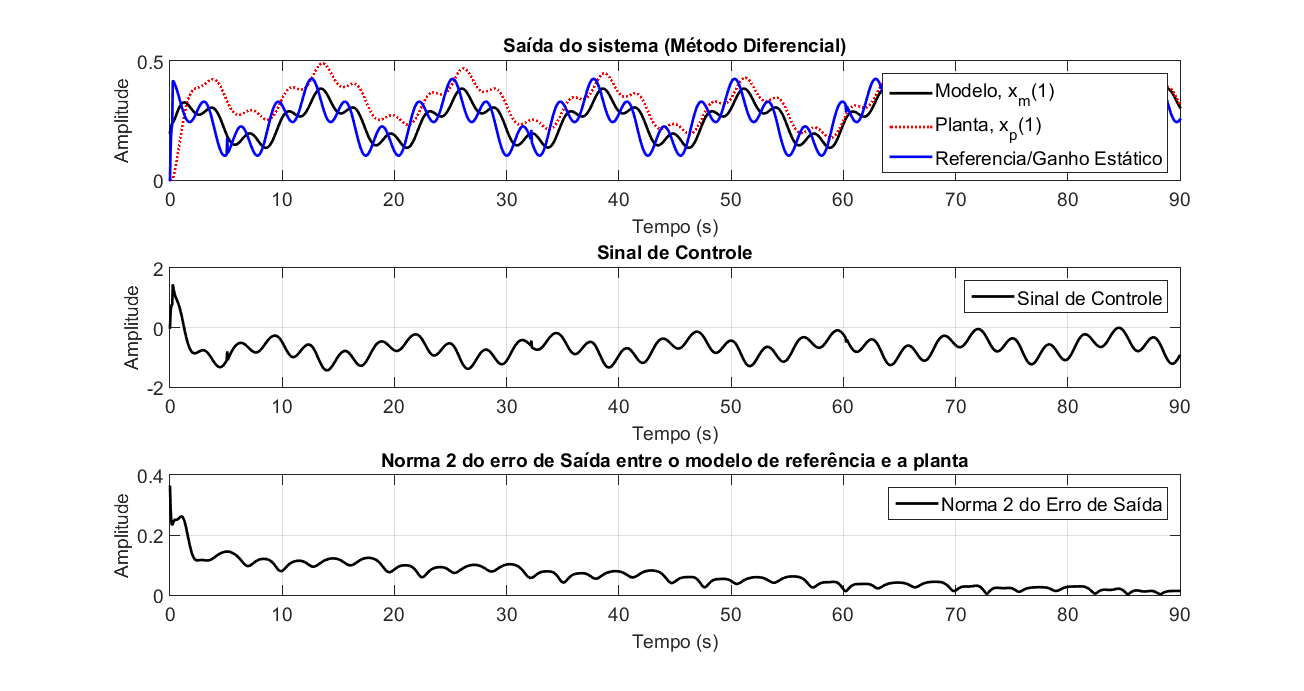
\includegraphics[width=0.62\linewidth]{./pics/SIM1_L1AA.png}
  \caption{Planta com ${\theta_p^*}^T = [2.3~~-3.6]$, ${\theta_m^*}^T = [-4~~-4]$, ${\theta_1}^T(0)=[-3 -2] $ }
\end{figure}
\end{frame}


\subsection{Controle Adaptativo por Modelo de Referência Indireto com Adaptação de Segundo Nível}

\begin{frame}
\frametitle{Localização de ${\theta_p}^*$}

Em \cite{han1}, foi provado que, se o vetor de parâmetros desconhecidos ${\theta_p}^*$ da planta estiver contido no fecho convexo $S$ dos parâmetros iniciais $\theta_i(0)$ de N modelos (onde $N\geq n+1$), ${\theta_p}^*\in S~~\forall t$, desde que $x_i(0)=x_p(0), \forall i$.\\

\end{frame}

\begin{frame}
\frametitle{Região Convexa}

\centering
\begin{figure}
  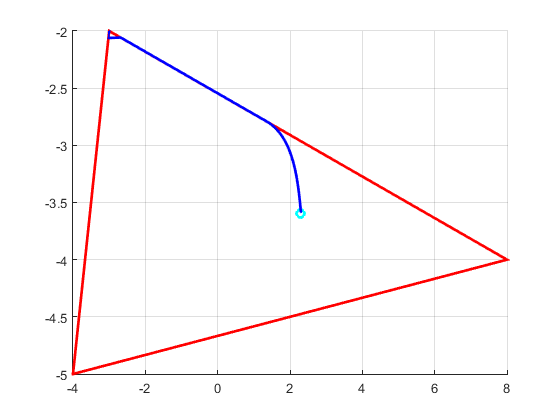
\includegraphics[width=.4\linewidth]{./pics/SIM1_Traj.png}
    \captionof{figure}{Em vermelho um fecho convexo no $\Re^2$, delimitado por [-4 -5], [-3 -2] e [8 -4]}
    \label{fig:test2912}
\end{figure}


\end{frame}
\begin{frame}
\frametitle{Múltiplos Modelos}

Seja o conjunto de modelos de identificação descritos por:

\begin{equation*}
\Sigma_i: \dot{\hat{x}}_i = A_m\hat{x}_i(t) + [A_i(t)-A_m]x_p(t) +bu(t)
\end{equation*}

Faremos uso da propriedade do fecho convexo para criar um modelo virtual a partir de uma combinação linear dos parâmetros dos modelos $\Sigma_i$. Por praticidade, usaremos o número mínimo de modelos $N=n+1$ daqui em diante.

\end{frame}

\begin{frame}

Tendo em mente como discutido anteriormente que:


\centering
\begin{minipage}{.48\textwidth}
  \flushleft
\begin{equation*}
\sum_{i=1}^{n+1}\alpha_i\theta_i(t) = \theta_p
\end{equation*}
\begin{equation*}
\sum_{i=1}^{n+1}\alpha_i\phi(t_0)=0
\end{equation*}
\begin{equation*}
\sum_{i=1}^{n+1}\alpha_i = 1
\end{equation*}
\end{minipage}%
  \hfill
\begin{minipage}{.48\textwidth}
  \flushright


\begin{equation*}
\theta_i(t_0) = \theta_{0}
\end{equation*}
\begin{equation*}
e_i(t_0)=0
\end{equation*}
\begin{equation*}
\dot{\theta}_i(t) = \dot{\phi}_i(t) = -{e_i}^T(t)Pbx_p(t)
\end{equation*}

\end{minipage}


\end{frame}


\begin{frame}

É possível enxergar as constantes $\alpha_1,\alpha_2,...,\alpha_{n+1}$ como uma alternativa de parametrização da planta. Consequentemente, a rapidez e precisão na estimação de $\alpha_i$ é que determinam seu desempenho.\\
\centering
\begin{minipage}{.48\textwidth}
  \centering
  \begin{equation*}
  \sum_{i=1}^{n+1}\alpha_i\theta_i(t) = \theta_p \space 
  \end{equation*}
\end{minipage}%
  \hfill

\begin{minipage}{.48\textwidth}
  \centering
    \begin{equation*}
    \sum_{i=1}^{n+1}\alpha_i e_i(t) = 0 \space
    \end{equation*}
\end{minipage}

\end{frame}

\begin{frame}
Em forma matricial:

\begin{equation*}
\bar{\Theta}(t)\bar{\alpha} = \theta_p
\end{equation*}
\begin{equation*}
\bar{E}(t)\bar{\alpha} = 0
\end{equation*}

onde $\bar{\Theta}$, $\bar{E} \in R^{n\times(n+1)}$

\end{frame}

\begin{frame}
Podemos então expressar:
\begin{equation*}
\Theta(t)\alpha = \theta_p - \theta_{n+1}
\end{equation*}
\begin{equation*}
E(t)\alpha = -e_{n+1}(t)
\end{equation*}

onde $\Theta(t)$, $E(t)\in R^{n\times n}$, onde cada vetor coluna é $\theta_i(t)-\theta_{n+1}(t)$ e $e_i(t)-e_{n+1}(t)$ respectivamente e $\alpha^T = [\alpha_1,...,\alpha_n]$. De onde obtemos a equação diferencial:

\begin{equation*}
\dot{\hat{\alpha}} = -\gamma E^T(t)E(t)\hat{\alpha} - \gamma E^T(t)e_{n+1}(t)
\end{equation*}

onde $\gamma$ é um escalar positivo.

\end{frame}


\begin{frame}
\frametitle{Figura de Mérito $\eta$}

Definimos a seguinte figura de mérito:

\begin{equation*}
\eta = \frac{\dot{\alpha}^T Q\dot{\alpha}}{1+\dot{\alpha}^T Q\dot{\alpha}}
\end{equation*}

E um escalar real:

\begin{equation}
d \in  ]0,1[
\end{equation}

Para $\eta\geq d$ a referência é PE. Se $\eta<d$ o valor do sinal de referência retorna assintoticamente para um valor constante.\\


\end{frame}



% ----------------- NOVO SLIDE --------------------------------
\section{Simulações com Modelos Fixos}
% % % % % % % % % % % % % % % % % % % % % % % % % % % % % % % % % % %
\subsection{Simulação 1, Segunda Ordem}
\begin{frame}
\centering
  \begin{minipage}{.48\textwidth}
  	\begin{figure}
  	 \centering
     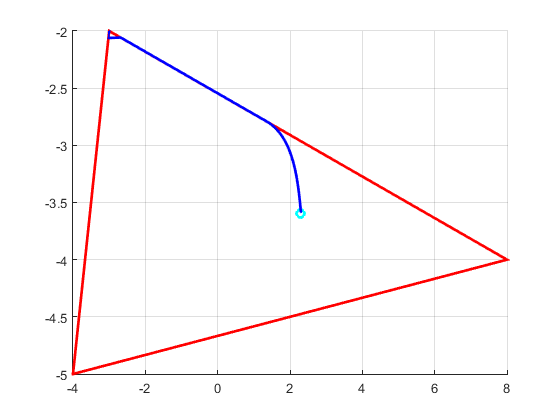
\includegraphics[width=0.8\linewidth]{./pics/SIM1_Traj.png}
     \caption{Trajetória dos parâmetros do modelo de identificação virtual em azul, fecho convexo delimitado pelos modelos de identificação nível 1 em vermelho}
  	\end{figure}
  \end{minipage}
  \hfill
  \begin{minipage}{.48\textwidth}
  	\begin{figure}
  	 \centering
     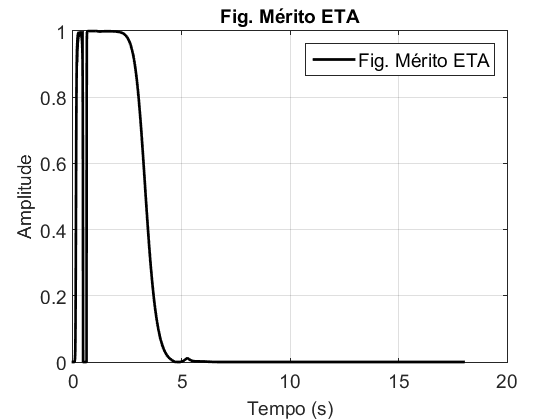
\includegraphics[width=0.8\linewidth]{./pics/SIM1_ETA.png}
     \caption{Comportamento da figura de Mérito $\eta$}
  	\end{figure}
  \end{minipage}
\end{frame}

\begin{frame}
\centering
  \begin{minipage}{.48\textwidth}
  	\begin{figure}
  	 \centering
     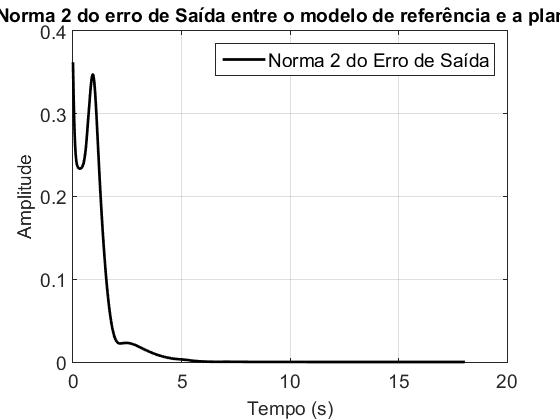
\includegraphics[width=0.8\linewidth]{./pics/SIM1_E0.png}
     \caption{Norma do vetor de erros de saída}
  	\end{figure}
  \end{minipage}
  \hfill
  \begin{minipage}{.48\textwidth}
  	\begin{figure}
  	 \centering
     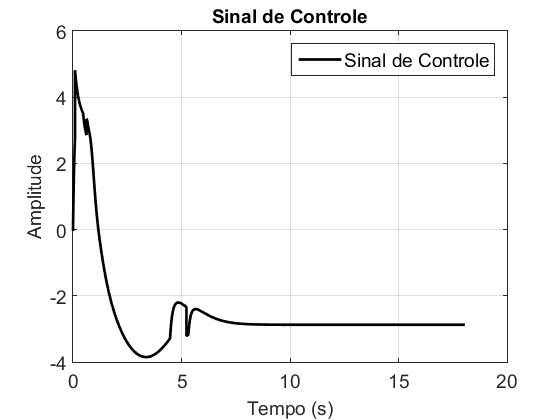
\includegraphics[width=0.8\linewidth]{./pics/SIM1_SinalCont.png}
     \caption{Sinal de Controle}
  	\end{figure}
  \end{minipage}
\end{frame}

\begin{frame}
\begin{figure}[!hbpt]
  \centering
  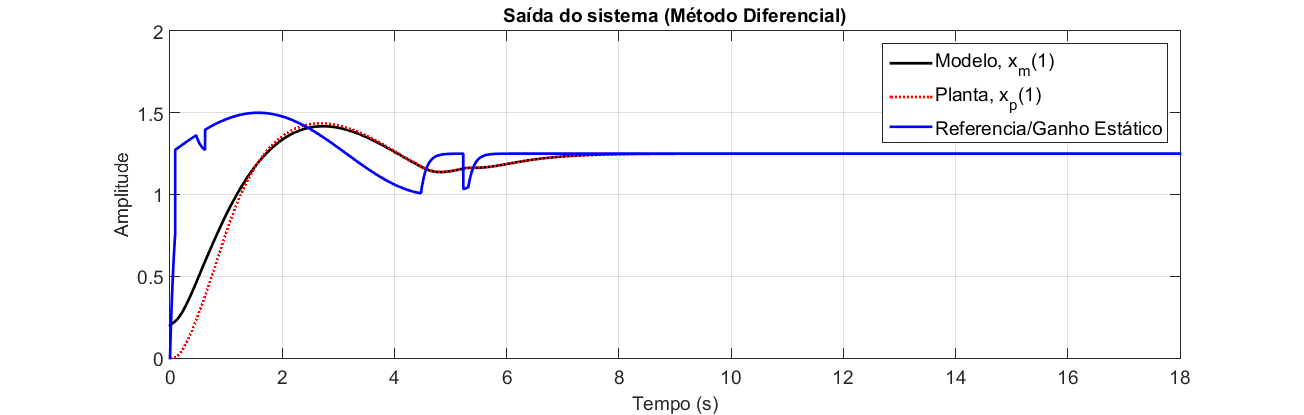
\includegraphics[width=\linewidth]{./pics/SIM1_Saida.png}
  \caption{Comportamento da Saída da Planta, Referência/Ganho Estático e Saída do Modelo de Referência}
\end{figure}
\end{frame}

\subsection{Simulação 3, Segunda Ordem, Com Perturbação}
\begin{frame}
\centering
  \begin{minipage}{.48\textwidth}
  	\begin{figure}
  	 \centering
     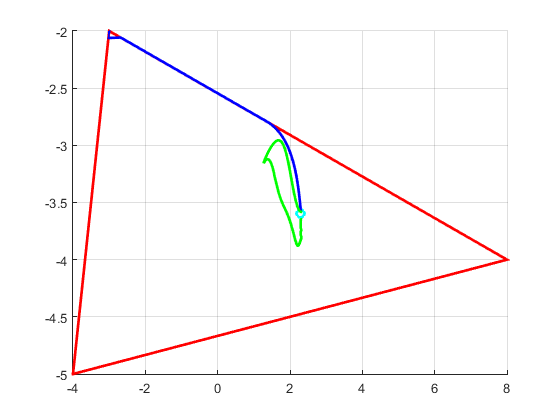
\includegraphics[width=0.8\linewidth]{./pics/SIM3_Traj.png}
     \caption{Trajetória dos parâmetros do modelo de identificação virtual em azul, e em verde após a inserção de uma perturbação, fecho convexo em vermelho}
  	\end{figure}
  \end{minipage}
  \hfill
  \begin{minipage}{.48\textwidth}
  	\begin{figure}
  	 \centering
     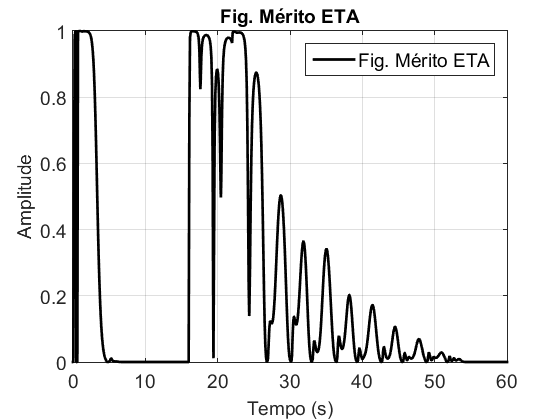
\includegraphics[width=0.8\linewidth]{./pics/SIM3_ETA.png}
     \caption{Comportamento da figura de Mérito $\eta$}
  	\end{figure}
  \end{minipage}
\end{frame}

\begin{frame}
\centering
  \begin{minipage}{.48\textwidth}
  	\begin{figure}
  	 \centering
     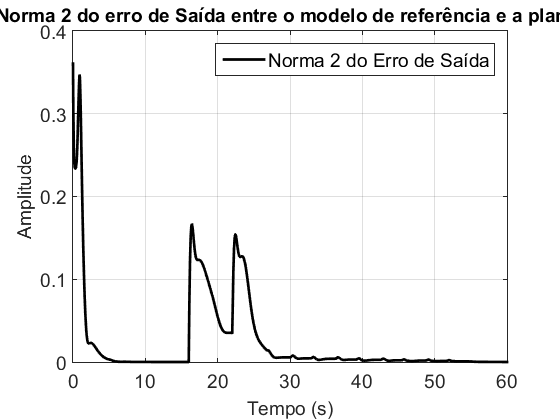
\includegraphics[width=0.8\linewidth]{./pics/SIM3_E0.png}
     \caption{Norma do vetor de erros de saída}
  	\end{figure}
  \end{minipage}
  \hfill
  \begin{minipage}{.48\textwidth}
  	\begin{figure}
  	 \centering
     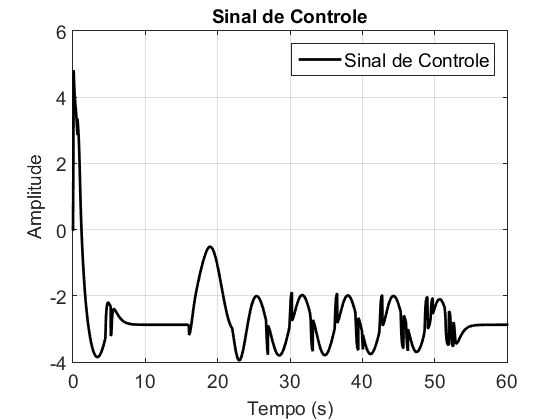
\includegraphics[width=0.8\linewidth]{./pics/SIM3_SinalCont.png}
     \caption{Sinal de Controle}
  	\end{figure}
  \end{minipage}
\end{frame}

\begin{frame}
\begin{figure}[!hbpt]
  \centering
  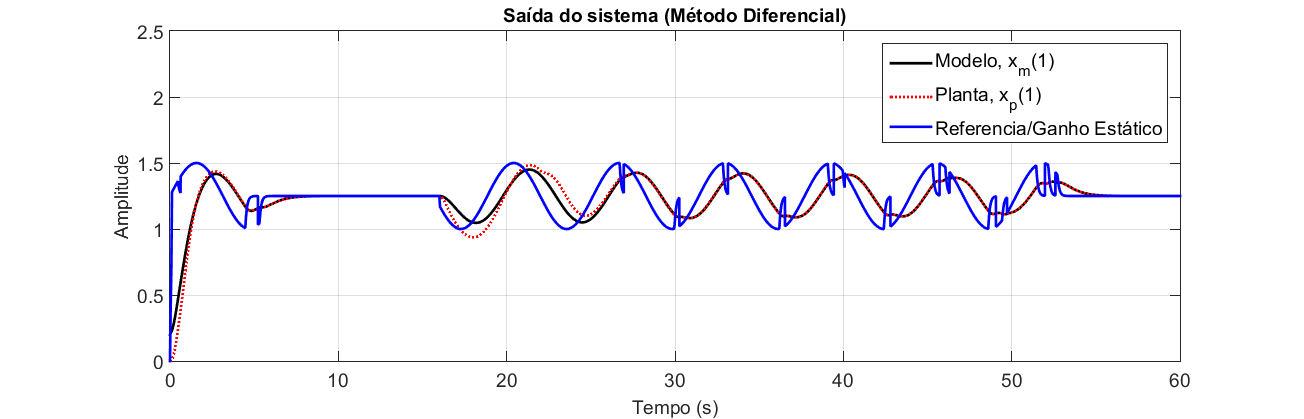
\includegraphics[width=\linewidth]{./pics/SIM3_Saida.png}
  \caption{Comportamento da Saída da Planta, Referência/Ganho Estático e Saída do Modelo de Referência}
\end{figure}
\end{frame}

\subsection{Simulação 4, Segunda Ordem, Com Ruído de Medição}
\begin{frame}
\centering
  \begin{minipage}{.48\textwidth}
  	\begin{figure}
  	 \centering
     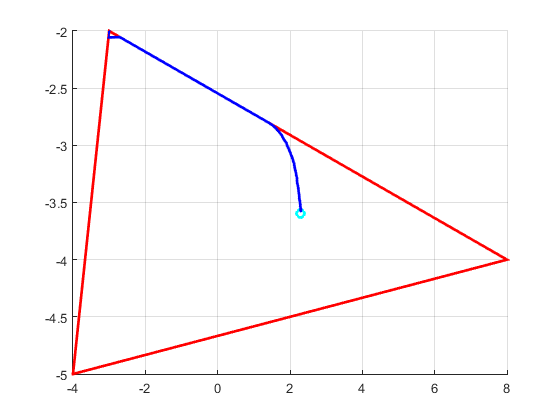
\includegraphics[width=0.8\linewidth]{./pics/SIM4_Traj.png}
     \caption{Trajetória dos parâmetros do modelo de identificação virtual em azul, fecho convexo delimitado pelos modelos de identificação nível 1 em vermelho}
  	\end{figure}
  \end{minipage}
  \hfill
  \begin{minipage}{.48\textwidth}
  	\begin{figure}
  	 \centering
     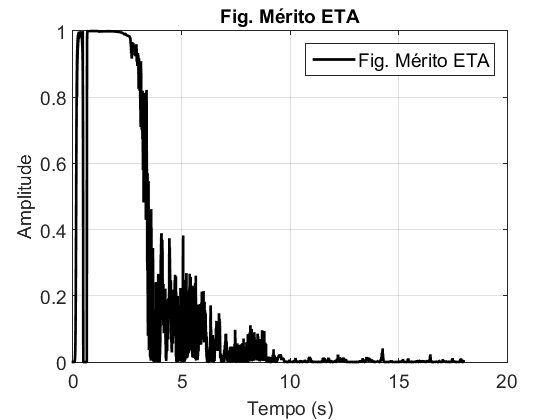
\includegraphics[width=0.8\linewidth]{./pics/SIM4_ETA.png}
     \caption{Comportamento da figura de Mérito $\eta$}
  	\end{figure}
  \end{minipage}
\end{frame}

\begin{frame}
\centering
  \begin{minipage}{.48\textwidth}
  	\begin{figure}
  	 \centering
     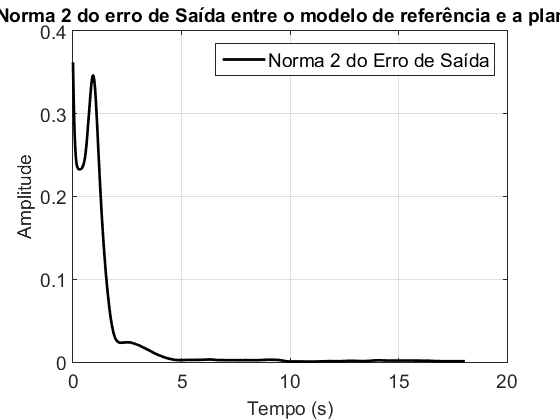
\includegraphics[width=0.8\linewidth]{./pics/SIM4_E0.png}
     \caption{Norma do vetor de erros de saída}
  	\end{figure}
  \end{minipage}
  \hfill
  \begin{minipage}{.48\textwidth}
  	\begin{figure}
  	 \centering
     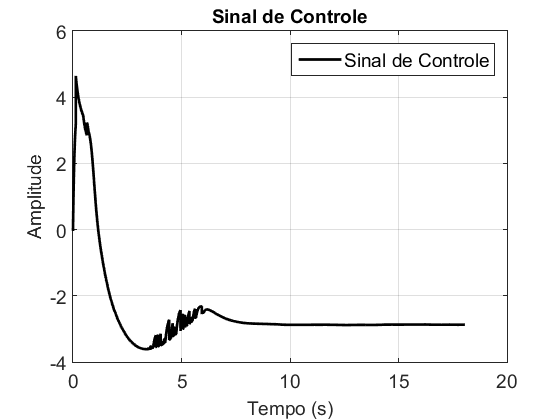
\includegraphics[width=0.8\linewidth]{./pics/SIM4_SinalCont.png}
     \caption{Sinal de Controle}
  	\end{figure}
  \end{minipage}
\end{frame}

\begin{frame}
\begin{figure}[!hbpt]
  \centering
  \includegraphics[width=\linewidth]{./pics/SIM4_Saida.png}
  \caption{Comportamento da Saída da Planta, Referência/Ganho Estático e Saída do Modelo de Referência}
\end{figure}
\end{frame}


% ----------------- NOVO SLIDE --------------------------------
\section{Conclusão}
\begin{frame}
\frametitle{Conclusão}

A Adaptação de Segundo Nível discutida para este artigo apresenta:

\begin{itemize}
\item[1] Boa rapidez de Convergência
\item[2] Robustez ao ruído
\item[3] Capacidade de rejeição de perturbação
\item[4] Compatibilidade com estratégias de Controle Indireto
\item[5] Necessidade de acesso completo ao vetor de estados da planta
\item[6] Limitação à plantas com $b$ conhecido e $A_p$ em forma companheira
\end{itemize}

Em trabalhos futuros trataremos das limitações apresentadas nos itens 5 e 6. Muito obrigado!

\end{frame}


% --- O comando \allowframebreaks ---
% Se o conteúdo não se encaixa em um quadro, a opção allowframebreaks instrui 
% beamer para quebrá-lo automaticamente entre dois ou mais quadros,
% mantendo o frametitle do primeiro quadro (dado como argumento) e acrescentando 
% um número romano ou algo parecido na continuação.
% --- O comando \allowframebreaks ---
% Se o conteúdo não se encaixa em um quadro, a opção allowframebreaks instrui 
% beamer para quebrá-lo automaticamente entre dois ou mais quadros,
% mantendo o frametitle do primeiro quadro (dado como argumento) e acrescentando 
% um número romano ou algo parecido na continuação.

%\begin{frame}
%\frametitle{Referências}
%\nocite{narendra1}
%\nocite{narendra_main}
%\nocite{narendra2012rationale}
%\nocite{narendra1997}
%\nocite{han1}
%\nocite{han2010}
%\nocite{han2012}
%\nocite{kuipers1}
%\nocite{ioannou2}
%\nocite{chen}
%nocite{ogata}
% %nocite{khalil}
%\end{frame}
% ----------------- FIM DO DOCUMENTO -----------------------------------------
\bibliography{bib-controleadaptativo}
\end{document}
